\documentclass{article}

\usepackage[a4paper]{geometry} % document dimensions
%\usepackage{amsmath} % multiline equation numbering
\usepackage{amssymb} % e.g. triangleq, checkmark
\usepackage{gensymb} % \degree symbol
%\usepackage{bm} % bold symbols numbering
\usepackage{authblk} % author/affiliation block
\usepackage[T1]{fontenc} % support accents via UTF

\usepackage{graphicx} % support for graphics
\usepackage[hidelinks, backref=page]{hyperref} % hyperlinks and autoref
\hypersetup{
    pdfauthor={Nick Ackerley},
    pdfsubject={Engineering Seismology},
    pdftitle={Open Model of Probabilistic Seismic Hazard Assessment for the Indian Subcontinent},
    pdfkeywords={seismology, hazard, India, OpenQuake}}
\usepackage{natbib} % bibliography support
\usepackage{caption} % support for captions
\usepackage{subcaption} % support for multiple figures with captions
%\providecommand*\hyphen{-} % dashed page numbers in bib

%\usepackage{multirow} % cells spanning rows in tables
%\usepackage{array} % vertically aligned table cells

\usepackage{enumitem} % control list formatting
\setlist[2]{nosep}

% allow figures to take up more of a page
\renewcommand{\floatpagefraction}{0.7}

% set up back-references
\renewcommand*{\backref}[1]{}
\renewcommand*{\backrefalt}[4]{%
    \ifcase #1 (Not cited.)%
    \or        (Cited on page~#2.)%
    \else      (Cited on pages~#2.)%
    \fi}
    
%%% PREAMBLE

\begin{document}

\title{Open Model of Probabilistic Seismic Hazard Assessment for the Indian Subcontinent}
\date{\today}

\setcounter{Maxaffil}{0} % compact author block
\author[1,2]{N. Ackerley}
\author[3]{G. Weatherill}
\author[3]{M. Pagani}
\affil[1]{Istituto Universitario di Studi Superiori, Pavia, Italy}
\affil[2]{Université Joseph Fourier, Grenoble, France}
\affil[3]{Global Earthquake Model (GEM), Pavia, Italy}

\maketitle

\begin{abstract}
Open models encourage peer review and collaboration; open models can be built upon.
\end{abstract}

\tableofcontents
\listoffigures
\listoftables

\section{Introduction}
\label{sec:Introduction}

\subsection{Overview}
\label{sec:Overview}

\subsection{Background}
\label{sec:Background}

We'll be adapting the model of \cite{nath2012probabilistic} to the OpenQuake platform.
\begin{figure*}
    \centering
    \begin{subfigure}[b]{0.48\textwidth}
        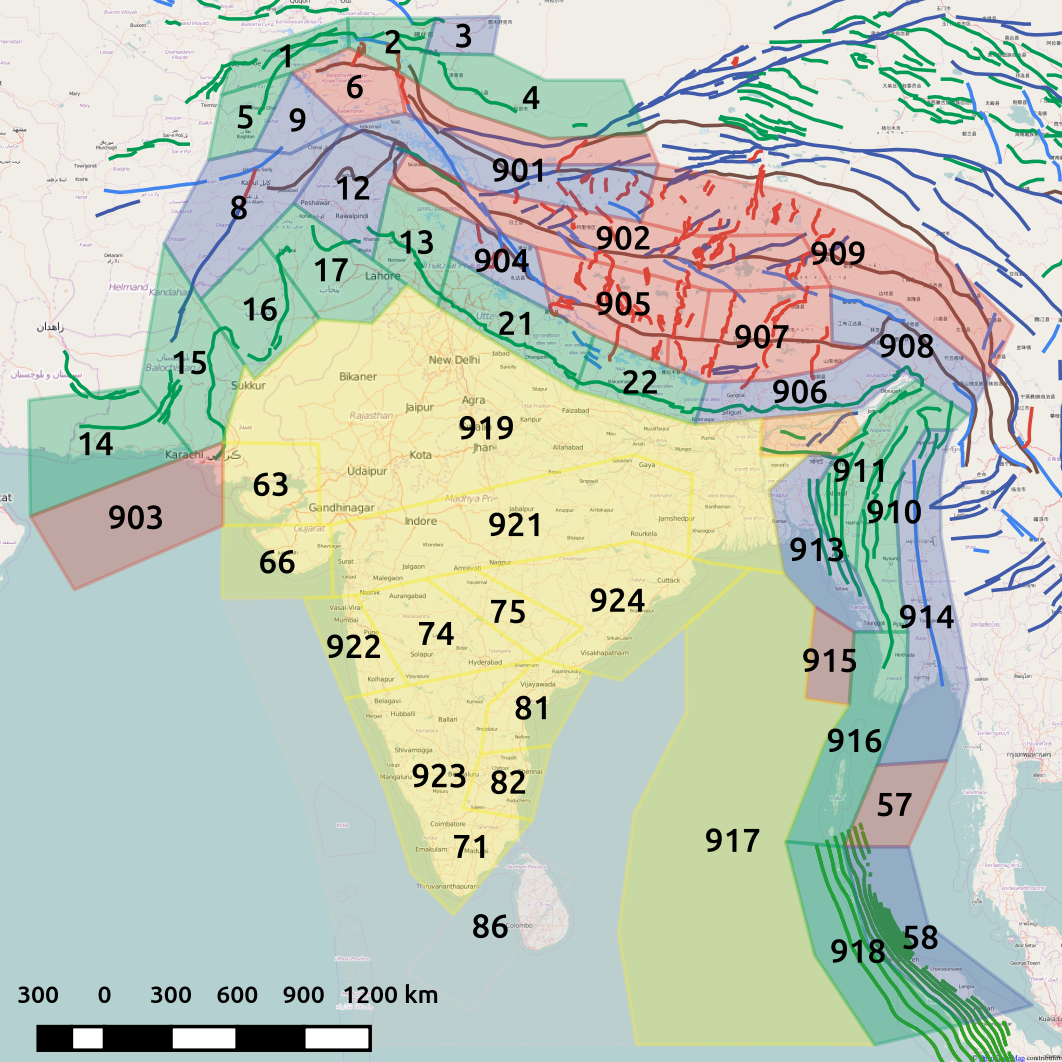
\includegraphics[width=\textwidth]{India_Areal_Layer_1.png}
        \caption[]{Layer 1}
        \label{fig:ArealLayer1}
    \end{subfigure}
    \begin{subfigure}[b]{0.48\textwidth}  
        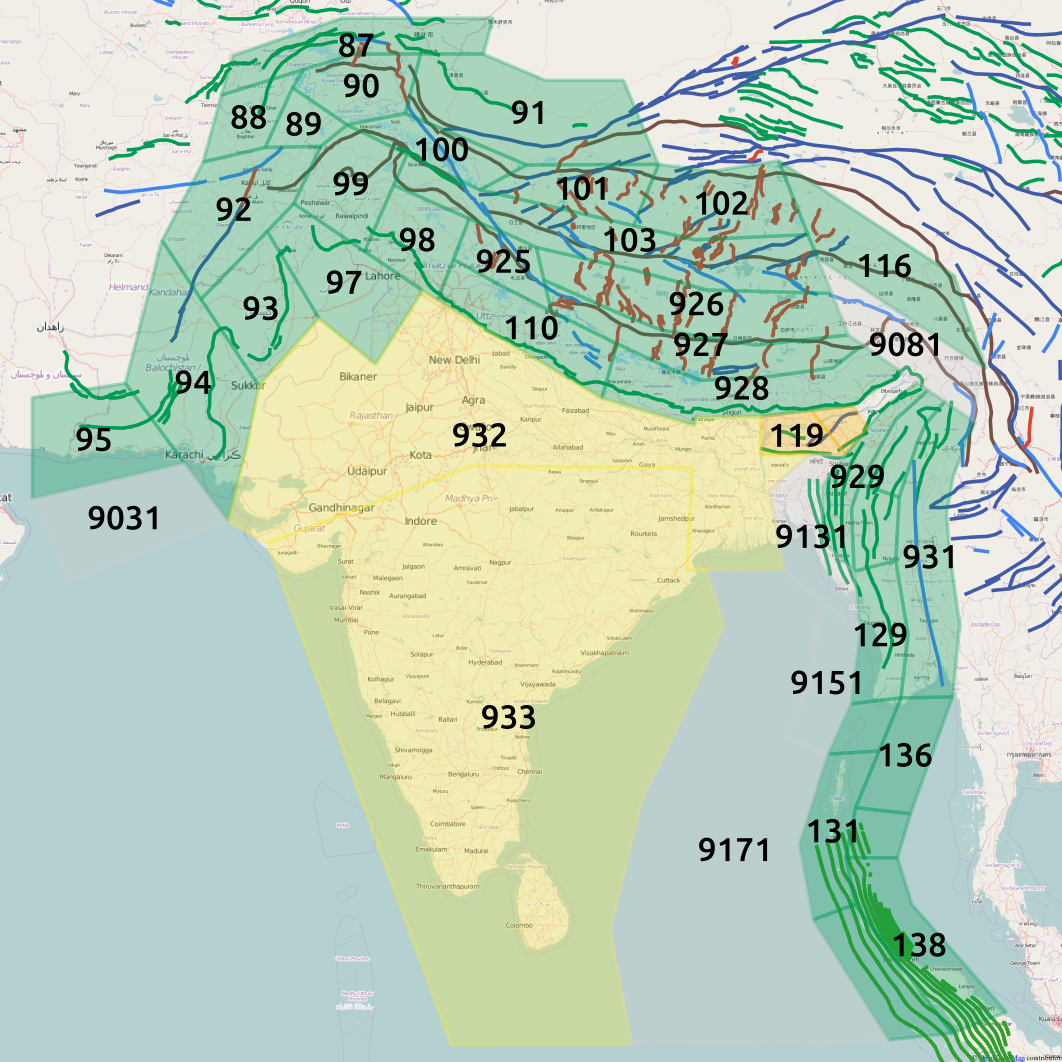
\includegraphics[width=\textwidth]{India_Areal_Layer_2.png}
        \caption{Layer 2}
        \label{fig:ArealLayer2}
    \end{subfigure}
    \vskip\baselineskip
    \begin{subfigure}[b]{0.48\textwidth}   
        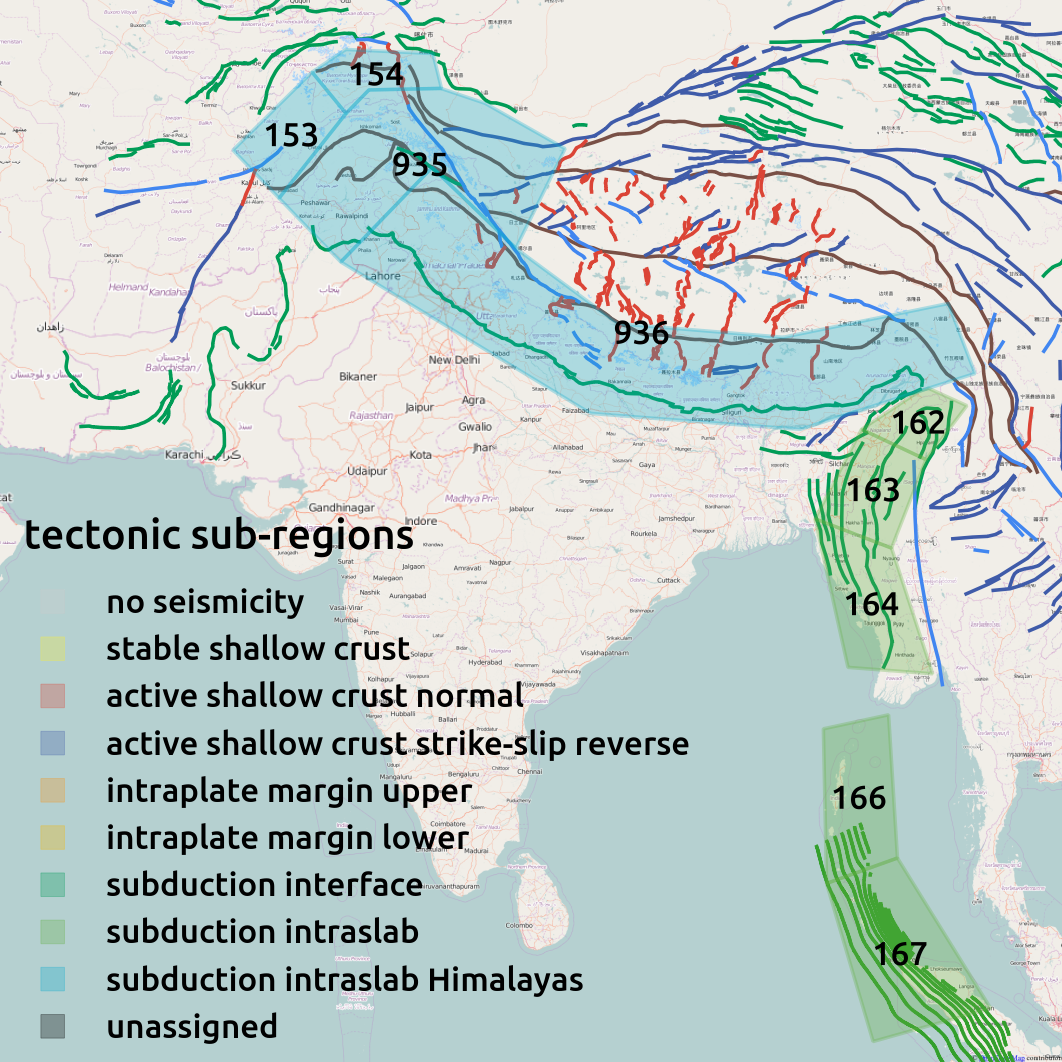
\includegraphics[width=\textwidth]{India_Areal_Layer_3.png}
        \caption{Layer 3}
        \label{fig:ArealLayer3}
    \end{subfigure}
    \begin{subfigure}[b]{0.48\textwidth}   
        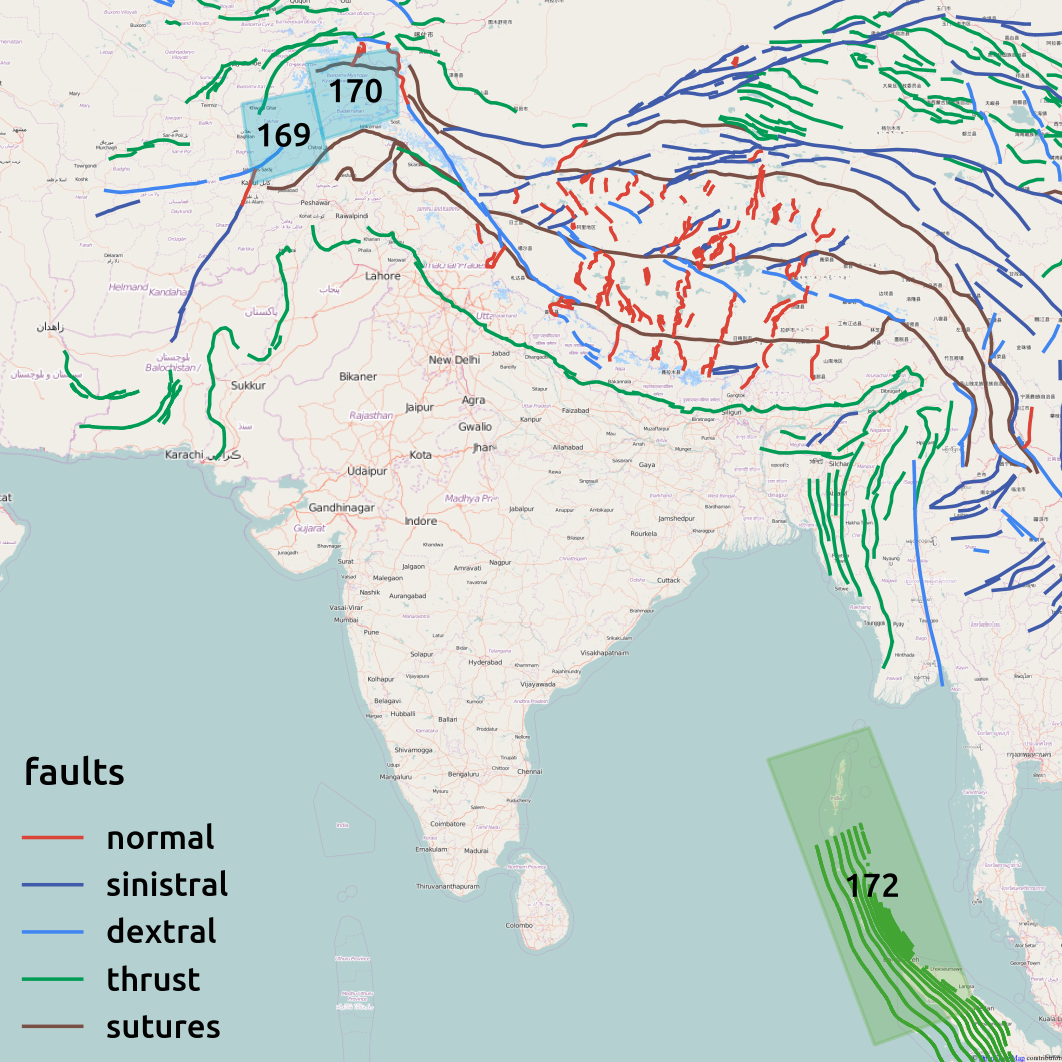
\includegraphics[width=\textwidth]{India_Areal_Layer_4.png}
        \caption{Layer 4}
        \label{fig:ArealLayer4}
    \end{subfigure}
    \caption[Tectonic region assignments for areal source model]
    {Tectonic region assignments for areal source model} 
    \label{fig:ArealSourceModel}
\end{figure*}

\section{Model implemetation}
\label{sec:Model}

\subsection{Seismogenic sources}
\label{sec:Sources}

\cite{thingbaijam2012seismogenic}

\subsubsection{Areal sources}
\label{sec:Areal}

As we will see in \autoref{subsubsec:GmpeWeights} ground motion prediction logic trees depend on correct assignment of tectonic region types. The main difficulty in implementing the areal source model of  \cite{nath2012probabilistic} was that although the intentions were generally clear, these assignments were not made explicit. The inferred tectonic region assignments assumed are shown in \autoref{fig:ArealSourceModel}.

Potentially problematic tectonic region type assignments:
\begin{itemize}
\item region 906 in the Great Himalayas just north of the Shillong plateau was assigned ``active shallow crust strike-slip reverse'' even though the main trace of the Himalayan subduction fault runs through it, because the dominant fault mechanism is strike-slip. 
\end{itemize}

An aspect ratio of 2 was furthermore assumed.

The seismogenic depth was assumed to be midway between the minimum and maximum. Is this justified by \cite{thingbaijam2012seismogenic}? Could it stand further refinement?


\subsubsection{Smoothed seismicity}
\label{sec:Smoothed}

\subsection{Ground-motion prediction}
\label{sec:GroundMotion}

\cite{sharma2009ground} points out that the decay rate of PGA for shallow India-Bangladesh and deep India-Burma border events have different distance scaling. The former leads to the necessity of a GMPE specific to the Shillong plateau \cite{nath2012ground} while the latter means interface subduction events need to be treated differently. 

Issues encountered while implementing GMPE logic tree:
\begin{itemize}
\item Layer 4 depth range of 180-300 km is significantly deeper than deepest events used in regression for ATBO03 (100 km), LILE08 (161 km), ZHAO06 (120 km) and GUPT10 (148 km) are specified for. YCSH97 only included events to 229 km. KANN06 is specified to 200 km depth, but is only used for interface events (layer 2).
\item Assumed “and Andaman-Sumatra subduction” missing from Figure 3.
\item Why is Youngs (1997) not used in the subduction interfaces?
\item Should the Japan/Cascadia distinction not also be used for interface subduction with Atkinson \& Boore (2003)?
\item \cite{nath2012probabilistic} doesn't seem to me to follow the recommendations of \cite{nath2011peak} as far as having two subduction intra-slab sub-regions: the former uses Indo-Myanmar and Himalayas while the latter recommends Indo-Myanmar and Hindukush. \cite{nath2012probabilistic} is followed strictly for for phase 1.
\item Assignment of source mechanism (normal or not, matters in shallowest layer only) is tricky.  Dip cannot be used to distinguish normal and reverse subduction because the subduction interface angle is not known. different GMPEs use different rake thresholds; a threshold of 30\degree\space was chosen, consistent with \cite{boore2008ground, campbell2008nga} but not \cite{zhao2006attenuation}.
\end{itemize}

Issued encountered while implementing GMPEs:

\cite{sharma2009ground}
\begin{itemize}
\item lacks a $M^2$ term \cite{cotton2006criteria}
\item does not define rock vs. soil
\end{itemize}

\cite{raghukanth2007estimation}
\begin{itemize}
\item typographical errors in coefficient tables: grossest error fixed, 3 other errors causing approximately 10\% error not fixed
\item actually defines 4 different models: must assume that for all of peninsular India was used by \cite{nath2012probabilistic}, not one of those for sub-regions.
\end{itemize}


\begin{table}
\caption[Ground shaking intensity models]{Ground shaking intensity models. Models newly implemented in OpenQuake as part of the current work are indicated.}
\centering
\begin{tabular}{c c l}
\hline
 Code & New & Reference \\
\hline
 AKBO10 & & \cite{akkar2010empirical} \\
 BOAT08 & & \cite{boore2008ground} \\ 
 CABO08 & & \cite{campbell2008nga} \\ 
 ZHAO06 & & \cite{zhao2006attenuation} \\ 
 ATBO03 & & \cite{atkinson2003empirical} \\ 
 ATMA09 & & \cite{atkinson2009predicted} \\ 
 LILE08 & & \cite{lin2008ground} \\ 
 YCSH97 & & \cite{youngs1997strong} \\ 
 TORO02 & & \cite{toro2002modification} \\ 
 ATBO06 & & \cite{atkinson2006earthquake} \\ 
 CAMP03 & & \cite{campbell2003prediction} \\ 
 SDBK09 & \checkmark & \cite{sharma2009ground} \\
 RAIY07 & \checkmark & \cite{raghukanth2007estimation} \\
 NTMN12 & \checkmark & \cite{nath2012ground} \\
 GUPT10 & \checkmark & \cite{gupta2010response} \\
 KNMF06 & \checkmark & \cite{kanno2006new} \\
\hline
\end{tabular}
\end{table}

\subsection{Logic Trees}
\label{subsec:Weights}

\subsubsection{Ground-Motion Prediction}
\label{subsubsec:GmpeWeights}

\cite{anbazhagan2015selection} seem to be proposing different weights for different regions based on single events in those regions. An extreme example is to define different weights for Anjar, 1956 and Bhuj , 2001 earthquakes even though the epicentres and depths were very close together. In contrast \cite{nath2011peak} compute LLH for 7 regions (using 38 events total) and state that, ``individual events do not have significant number of observations to support a viable ranking basis.''

\cite{anbazhagan2015selection} seem to misuse the concept of data support index (DSI) \citep{delavaud2012toward} by setting weights to zero when the DSI is negative. The threshold is arbitrary and is chosen without discussion. As \cite{delavaud2012toward} point out ``more important
than the sign of the DSI is the difference of DSI between
two models.''

Both \cite{anbazhagan2015selection} and \cite{nath2011peak} rely on estimating ground motions from macroseismic intensity. I'm sure it is a matter of low seismicity and lack of instrumentation, but I'm still surprised. I would expect the catalogue for peninsular India to be complete for 20 years to magnitude 5 so that one could thus get 10 well-recorded events, at least. There is significant additional (aleatory and epistemic) variability in mapping EMS to PGA which must obscure the true performance of the GMPEs.  Perhaps this is part of why  \cite{anbazhagan2015selection} and \cite{nath2011peak} arrive at such different LLH scores and rankings for the same events \cite[][Table 5]{anbazhagan2015selection}. It would be interesting to compare the results of LLHs computed using EMS inferred from digitized intensity maps to those computed using instrumental PGA for at least a few events since 1990. \cite{nath2011peak} take a step towards this by looking at the scatter in their mapping of PGA to EMS but it's not quite the same.

Many authors \citep{scherbaum2009model, nath2011peak, delavaud2012toward, anbazhagan2015selection} seem unduly interested in "ranking", i.e.  constructing an ordered list of GMPEs. This is not a horse race. \cite{scherbaum2009model} suggests a way to turn an LLH score into a logic-tree weight and the formula does not require ranking. Furthermore, in constructing a logic tree one must include factors outside the performance-based scoring, for example an assessment of whether the set is ``mutually exclusive and collectively exhaustive'' \citep{bommer2008use}. For me the question of ranking is just "noise" which obscures more important questions.

The mutual exclusivity requirement means, to me, that models should be omitted which are redundant in the sense of being too similar to other models in terms of the methodology of their construction, especially if that means they make similar predictions and have similar limitations as a result. For example the exclusion of models which have been superseded \citep{cotton2006criteria} can be seen as an application of the requirement that models be mutually exclusive. Another example would be, for a GMPE logic tree intended for the Indian subcontinent, to omit a model such as \cite{hwang1997attenuation} in favour of \cite{atkinson2006earthquake} since both are based on stochastic simulation in Eastern North America.

The collective exhaustiveness requirement means, is trickier. It is this requirement which pushes hazard modellers to seek out and evaluate more and complementary types of models. Thus models with broad data support from other regions complement models with poor data support from the target region. Stochastic models supplement data-driven models. Models with different functional forms, distance or magnitude ranges can complement each other.

The process of developing a logic tree to assess epistemic uncertainty is thus a dialectical one. Mutual exclusivity and collective exhaustiveness comprise opposing forces which must be exerted alternately and in tandem.

[Now apply these principles to move forward from \cite{nath2012probabilistic}!] 

\subsubsection{Source Models}
\label{subsubsec:SourceModelWeights}

\section{Hazard results}
\label{sec:Hazard}

\subsection{Verification}
\label{sec:Verification}

\subsection{Sensitivity}
\label{subsec:Sensitivity}

\section{Conclusions}
\label{sec:Conclusions}

\section*{Acknowledgement}
Acknowledgements here



\bibliographystyle{apalike}
\bibliography{/home/nick/Desktop/Library/PSHA.bib}

\end{document}
